\documentclass[conference]{IEEEtran}
\IEEEoverridecommandlockouts
% The preceding line is only needed to identify funding in the first footnote. If that is unneeded, please comment it out.
\usepackage{cite}
\usepackage{amsmath,amssymb,amsfonts}
\usepackage{algorithmic}
\usepackage{graphicx}
\usepackage{textcomp}
\usepackage{xcolor}
\usepackage[FIGTOPCAP]{subfigure}
\def\BibTeX{{\rm B\kern-.05em{\sc i\kern-.025em b}\kern-.08em
    T\kern-.1667em\lower.7ex\hbox{E}\kern-.125emX}}

\makeatletter
\newcommand{\linebreakand}{%
\end{@IEEEauthorhalign}
\hfill\mbox{}\par
\mbox{}\hfill\begin{@IEEEauthorhalign}
}


\begin{document}

\title{Deep Neural Networks for Assessing the \\ Age of Majority from\\ Panoramic Dental X-ray Images\\

\thanks{Identify applicable funding agency here. If none, delete this.}
}

\author{
	
		\IEEEauthorblockN{Antonio Jos\'e Aragon Molina}
	\IEEEauthorblockA{\textit{Department of Computer Science} \\
		\textit{Universit\`a degli Studi di Milano}\\
		Milano, Italy \\
		antonio.aragon@unimi.it}
	\and
	\IEEEauthorblockN{Danilo De Angelis}
	\IEEEauthorblockA{\textit{Department of
			Biomedical Sciences for Health} \\
		\textit{Universit\`a degli Studi di Milano}\\
		Milano, Italy \\
		danilo.deangelis@unimi.it}
	\and
		\IEEEauthorblockN{Ruggero Donida Labati}
	\IEEEauthorblockA{\textit{Department of Computer Science} \\
		\textit{Universit\`a degli Studi di Milano}\\
		Milano, Italy \\
		ruggero.donida@unimi.it}
	\linebreakand 	
	\IEEEauthorblockN{Fabio Scotti}
	\IEEEauthorblockA{\textit{Department of Computer Science} \\
		\textit{Universit\`a degli Studi di Milano}\\
		Milano, Italy \\
		fabio.scotti@unimi.it}
	\and 
	\IEEEauthorblockN{Vincenzo Piuri}
	\IEEEauthorblockA{\textit{Department of Computer Science} \\
		\textit{Universit\`a degli Studi di Milano}\\
		Milano, Italy \\
		vincenzo.piuri@unimi.it}	
}
\maketitle

\begin{abstract}
Forensic anthropologists and odontologists frequently need to establish the age of a living or deceased individual. In particular, a relevant problem consists of determining the age of majority for persons not possessing identity documents or for whom it's not possible to have trustworthy information on their date of birth. An accurate technique to perform this measurement involves the analysis of panoramic dental X-ray images (orthopantomography), conducted by experienced forensic scientists. Although studies in the literature on automatic methods for age estimation based on dental images present promising results, none of them specifically focus on establishing the age of majority. Instead, we propose a method based on deep learning for assessing the age of majority. Specifically, we consider the age of majority as 18 years and propose a method that mimics the analysis performed by human experts by examining the third molars with Convolutional Neural Networks (CNNs). The proposed method can assess the age of majority from a single or multiple molar images. To this end, we investigated a feature-level as well as a score-level fusion strategy. We assessed the performance of the proposed method using a specifically collected dataset composed of 236 samples from individuals ranging from 15 to 22 years old. We compared the obtained results with classifications performed by an expert forensic odontologist, achieving similar accuracy, thus proving the applicability of our method as a decision support tool for forensic scientists.
\end{abstract}

\begin{IEEEkeywords}
Age, dental biometrics, convolutional neural networks, forensics
\end{IEEEkeywords}

\section{Introduction}
Forensic anthropologists and odontologists are frequently asked to estimate the age of living or deceased individuals. In this context, one of the most relevant problems consists of assessing the age of majority for persons not possessing legal documents. This problem is particularly significant since regulations are usually different for underage and adult persons. However, assessing the age of majority could be a particularly difficult task, especially if the real age of the individual is just slightly lower or higher than the legal age. In this case, even assessments performed by experienced scientists could be erroneous (human error). In this paper, we consider the legal age threshold as 18 years, since this value is used in a wide number of countries.


\begin{figure*}[!t]
	\centering
	\subfigure[]{\includegraphics[width=0.37\textwidth]{img/16_f.eps}}
	\subfigure[]{\includegraphics[width=0.37\textwidth]{img/21_f.eps}}\\
	\subfigure[]{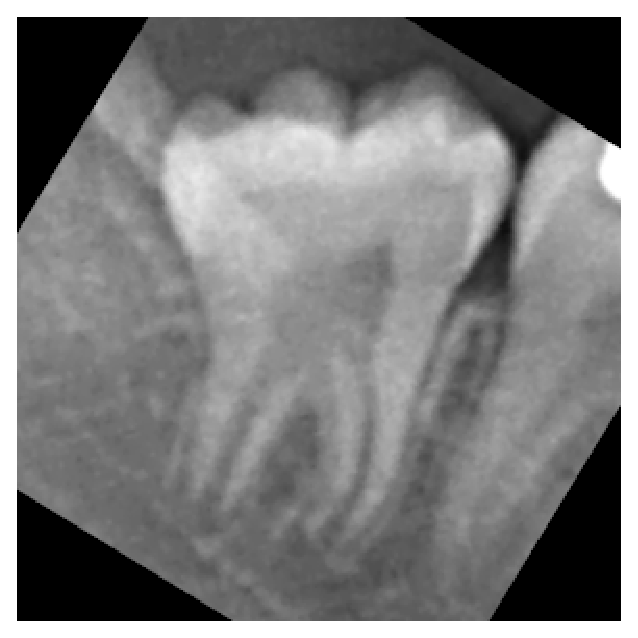
\includegraphics[width=0.18\textwidth]{img/16_dx.eps}}
	\subfigure[]{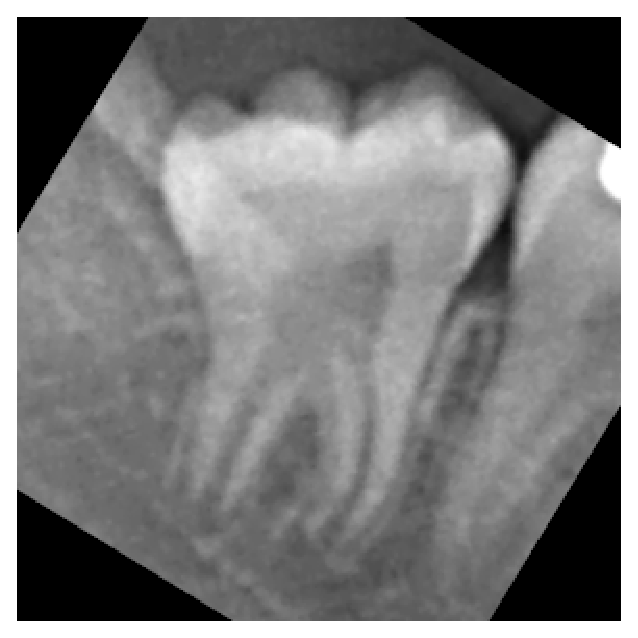
\includegraphics[width=0.18\textwidth]{img/16_dx.eps}}	
	\subfigure[]{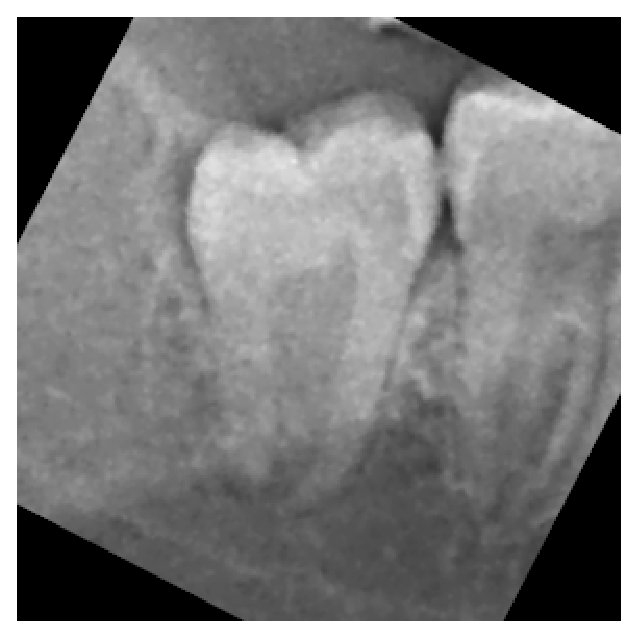
\includegraphics[width=0.18\textwidth]{img/21_dx.eps}}
	\subfigure[]{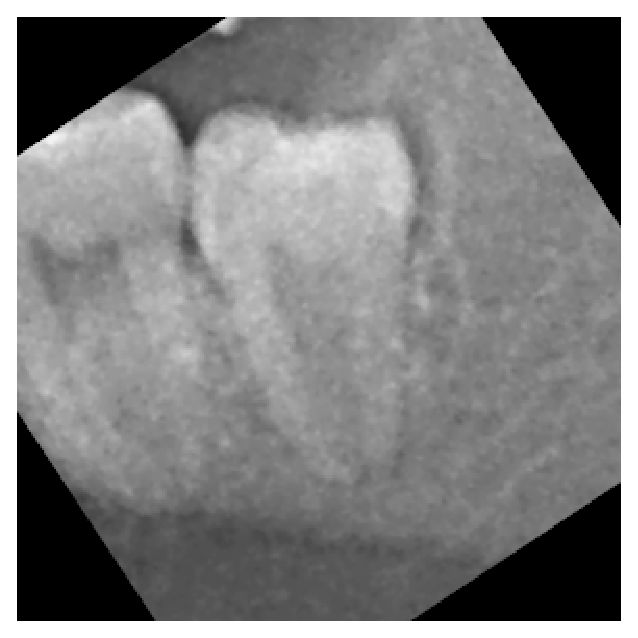
\includegraphics[width=0.18\textwidth]{img/21_sx.eps}}
	\caption{Examples of orthopantomography images and images of third molars of the inferior arch: a) orthopantomography image acquired from a 16 years old individual; b) orthopantomography image acquired from a 21 years old individual; c) and d) enahnced regions of a) depicting the third molars of the inferior arch; e) and f) enahnced regions of b) depicting the third molars of the inferior arch. While the size of teeth is different between subjects, the shape of the third molars is different for underage and adult individuals.}
	\label{figDenti}
\end{figure*}


Forensic anthropologists and odontologists frequently perform age assessment by analyzing orthopantomography images. Specifically, scientists evaluate the growth stage of every tooth using well-established approaches in the literature. Relevant approaches are the staging techniques proposed by Demirjian \cite{Demirjian} and Moorees \cite{Moorees}. Considering the age of majority as equal to 18 years, the most relevant information is represented by the growth stage of the third molars. Many forensic anthropologists and odontologists, therefore, perform the age of majority assessment by analyzing only the portions of images representing the third molars. Specifically, they frequently consider only the third molars of the inferior arch since they are more visible compared to the ones of the upper arch. Fig.~\ref{figDenti}a shows an orthopantomography image acquired from a 16-year-old individual, while Fig.~\ref{figDenti}b shows an orthopantomography image acquired from a 21-year-old individual. Fig.~\ref{figDenti}c and Fig.~\ref{figDenti}d show enhanced regions of Fig.~\ref{figDenti}a depicting the third molars of the inferior arch. Fig.~\ref{figDenti}e and Fig.~\ref{figDenti}f show enhanced regions of Fig. 1b depicting the third molars of the inferior arch. While the size of teeth is different between subjects, the shape of the third molars is different for underage and adult individuals.

In the literature, there are various studies on age estimation from orthopantomography images \cite{survey}. However, to the best of our knowledge, only one study evaluates whether the age estimated from an orthopantomography image is greater than 18 years \cite{PMID33661340}. This study considers only a single tooth as the input sample and has been evaluated using a dataset of samples acquired from individuals ranging from 5 to 24 years old, thus not representing the typical application scenario for which forensic scientists are asked to assess the age of majority.

We propose a method based on deep neural networks designed to emulate the age assessment performed by forensic scientists. Specifically, the proposed method takes as input a single or multiple images of the third molars and returns a Boolean representing adulthood reaching. To search for the best configuration of the proposed method for data collected in real application conditions, we investigated different neural models and fusion strategies. Specifically, we implemented a feature-level and a score-level fusion strategy.

To evaluate the proposed method, we collected a dataset of orthopantomography images simulating cases for which forensic odontologists are asked to assess the age of majority in real life. Specifically, we cooperated with Italian hospitals in collecting a dataset of dental radiographs from 236 individuals, ranging from 16 to 22 years old. The performed tests showed that the proposed method obtained remarkable results, with a classification accuracy of xxx\%. We also compared the obtained results with those of a forensic odontologist, obtaining similar accuracy.


This paper presents the following contributions:
\begin{itemize}
\item To the best of our knowledge, it is the first paper on an automatic method for legal age assessment designed to evaluate multiple regions of orthopantomography images.
\item To simulate real conditions for which forensic odontologists are asked to assess the age of majority, we collected a dataset of samples from individuals in a similar age range (ranging from 15 to 22 years old) and validated the proposed method on the collected data.
\item To validate the applicability of the proposed automatic method for assessing the age of majority, we compared the performance of our method with estimations performed by an expert forensic odontologist, obtaining similar results.
\end{itemize}

The proposed method could represent a valid decision support tool for forensic science since our method obtained relevant accuracy, comparable to that of a forensic odontologist.
This paper is organized as follows: Section II describes the state of the art on age estimation from dental radiographs. Section III presents the proposed method. Section IV describes the collected dataset, performed tests, and obtained results. Section V concludes the work.



\section{Related Work}


Dental anatomy is a distinctive biometric trait frequently analyzed by forensic odontologists to verify the identity of living or deceased individuals, or to infer soft biometric characteristics \cite{DonidaLabati2019} such as age and biological sex.
In the literature, there are studies on automatic identity recognition techniques \cite{jainDenti}, as well as on the extraction of soft biometric characteristics from dental data \cite{survey}.

Considering orthopantomography images, which are the most commonly available data for forensic scientists, there are studies on automatic methods for identity verification \cite{FAN2020110416}, tooth segmentation \cite{a6bd905adf2c48db8e08e228d114d9c4}, age estimation \cite{Alkaabi2020}, and biological sex evaluation \cite{8977504}.

Various methods for age estimation can be categorized based on statistical approaches \cite{8073563}, machine learning techniques utilizing handcrafted features \cite{SARIC2022111245}, or deep neural networks. Generally, methods employing deep neural networks tend to achieve higher accuracy compared to other approaches. Some studies rely on pre-trained Convolutional Neural Networks (CNNs) \cite{10.1007/978-3-658-33198-6_46}, while other approaches are based on ad-hoc CNNs \cite{MILOSEVIC2022116038, healthcare11081068}.

Age estimation methods are usually implemented as multiple-class classifiers, where each class represents a group of ages \cite{healthcare11081068, 0a72cc460005411bac3e72cd31862059}  or as regressors \cite{SARIC2022111245, PMID33661340, MILOSEVIC2022116038}. There is also a study on the classification of children under and over 13 years old \cite{10.1007/978-3-658-33198-6_46}. Furthermore, there is an automatic approach to estimate the development stage of single tooths \cite{egitto}.  
 

To the best of our knowledge, there is only one study in the literature reporting results on the age of majority estimation \cite{PMID33661340}. However, this study considers only a single tooth and has been tested for a dataset of samples collected from a wider set of ages compared to real forensic applications. In contrast, we propose a method capable of using multiple images of teeth to assess the age of majority, which has been evaluated for a dataset simulating data analyzed by forensic odontologists in real scenarios.

\section{Proposed Method}
SCHEMAS
\subsection{Preprocessing}
The proposed classifiers take as input one or more images representing the third molars in orthopantomography images. In this paper, we consider enhanced images of the third molars created by forensic odontologists.

The images of the third molars are obtained by cropping a fixed-size region of $290 \times 290$ pixels, centered at coordinates selected by a human operator. In cases where the third molar is missing, the center coordinates correspond to where the third molar was supposed to be. The third molar image is then rotated to align its major axis with the $y$ axis.

To simplify the segmentation and rotation processes, we developed a graphical user interface. This software also allows for the insertion of additional annotations to the images.

\section{Experimental Results}
\subsection{Dataset}

% Table generated by Excel2LaTeX from sheet 'Sheet1'
\begin{table}[t]
	\centering
	\caption{Dataset Composition}
	\begin{tabular}{cc}
		\hline
		\hline
		Years & Number of subjects \\
		\hline
		15    & 6 \\
		16    & 31 \\
		17    & 32 \\
		18    & 41 \\
		19    & 25 \\
		20    & 41 \\
		21    & 44 \\
		22    & 17 \\
		\hline
		\hline
	\end{tabular}%
	\label{tabDB}%
\end{table}%


\subsection{Comparison with Forensic Odontologists}
According to forensic odontologists, the most critical problem consists of assessing the age of majority for 17-year-old individuals since the third molars could be in a more advanced growing stage compared to the classification techniques proposed by Demirjian and Moorees.

For the considered dataset, an expert forensic odontologist erroneously classified $17\%$ of the 17-year-old individuals as older than 18 years old. In contrast, the proposed method achieved a better accuracy, with only $A\%$ classification error for the same samples.

This result demonstrates that deep neural networks can effectively be used by forensic scientists as decision support tools for assessing the age of majority, even for challenging data.

\section{Conclusion}


\bibliographystyle{IEEEtran}

\bibliography{biblio}\end{document}


\end{document}
